\subsection{de.view.elements}

\rule{\textwidth}{0.4pt} 
\class{CookieNotice}
public class CookieNotice

\begin{minipage}{0.3\textwidth}
    \begin{figure}[H]
        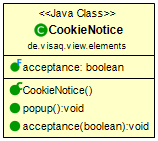
\includegraphics[scale = 0.6]{media/frontend/view/de.view.elements/CookieNotice_Class.png}
    \end{figure}
    \end{minipage} \hfill
    \begin{minipage}{0.6\textwidth}
Popup, welches den Benutzer darüber informiert, dass VisAQ Cookies nach dem EU Recht verwendet
\end{minipage}

Attribute:
\begin{itemize} 
    \item \emph{public final boolean acceptance} Ein boolean Attribut, welches verwendet wird um zu entscheiden ob der Benutzer die Cookies akzeptiert oder nicht. Ist der boolean positiv, so werden die Einstellungen auf der Seite des Clients gespeichert. Standardmäßig ist dieser Wert beim ersten Laden der Webapplikation negativ gesetzt.
\end{itemize}
Methoden:
\begin{itemize} 
    \item \emph{public CookieNotice()} Konstruktor für die CookieNotice 
    \item \emph{public popup()} Das Pupup Fenster welches beim laden der Webapplikation die CookieNotice anzeigt und dem Benutzer erlaubt die Cookies zu akzeptieren
    \item \emph{public void acceptance(boolean acceptance)} Speichert die Benutzerdaten des Benutzers auf desen Endgerät
\end{itemize}
